\begin{figure}[!h]
	\centering
	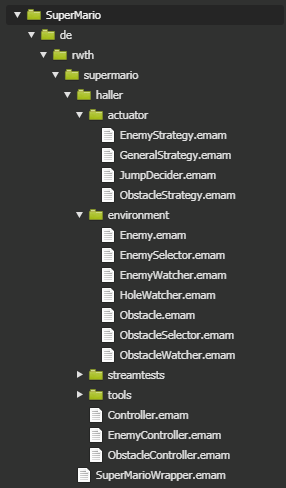
\includegraphics[scale=1]{pictures/haller_mariooutline.PNG}
	\caption{Supermario package outline}
	\label{fig:mariopackageoutline}
\end{figure}


\begin{lstlisting}[caption=SuperMarioWrapper.emam, morekeywords={package, stream, tick, for, ports, port, connect, component, in, out, instance, ->},
frame=single, basicstyle=\tiny]
package de.rwth.supermario;

import de.rwth.supermario.haller.Controller;

component SuperMarioWrapper {
    ports   
        in Z^{1,2} marioPosition,
        in Z^{1,2} marioVelocity,
        in Z marioHeight,
        in Z^{5,2} nextEnemyPositions,
        in Z^{5,2} nextObstaclePositions,
        in Z nextHole,
        in Z^{5,2} nextLootCrates,
        in Q tickSize,
        in Z marioResting,
        out Z(-1 : 1 : 1) marioDirection,
        out Z marioJump,
        out Z marioDown,
        out Z marioShoot;
        

    //Replace this with your own custom controller
    instance Controller controller;
    
    connect marioPosition -> controller.marioPosition;
    connect marioVelocity -> controller.marioVelocity;
    connect marioHeight -> controller.marioHeight;
    connect nextEnemyPositions -> controller.nextEnemyPositions;
    connect nextObstaclePositions -> controller.nextObstaclePositions;
    connect nextHole -> controller.nextHole;
    connect nextLootCrates -> controller.nextLootCrates;
    connect tickSize -> controller.tickSize;
    connect marioResting -> controller.marioResting;
    
    connect controller.marioJump -> marioJump;
    connect controller.marioDirection -> marioDirection;
    connect controller.marioDown -> marioDown;
    connect controller.marioShoot -> marioShoot;
    
}
\end{lstlisting}


\begin{lstlisting}[caption=SuperMarioWrapper.emam, morekeywords={package, stream, tick, for, ports, port, connect, component, in, out, instance, ->},
frame=single, basicstyle=\tiny]
package de.rwth.supermario.haller;


import de.rwth.supermario.haller.tools.OrRelation_3;
import de.rwth.supermario.haller.actuator.GeneralStrategy;
import de.rwth.supermario.haller.actuator.JumpFilter;
import de.rwth.supermario.haller.EnemyController;
import de.rwth.supermario.haller.ObstacleController;

component Controller {
    ports
        in Z^{1,2} marioPosition,
        in Z^{1,2} marioVelocity,
        in Z marioHeight,
        in Z^{5,2} nextEnemyPositions,
        in Z^{5,2} nextObstaclePositions,
        in Z nextHole,
        in Z^{5,2} nextLootCrates,
        in Q tickSize,
        in Z marioResting,
        out Z(-1 : 1 : 1) marioDirection,
        out Z marioJump,
        out Z marioDown,
        out Z marioShoot;
        
    //Sub-Controllers to keep this file clean and enhance overall modularity
    //This one deals with the enemies
    instance EnemyController enemyController;
    connect  nextEnemyPositions -> enemyController.nextEnemyPositions;
    
    //This one deals with pipes, staircases and holes
    instance ObstacleController obstController;
    connect  nextObstaclePositions -> obstController.nextObstaclePositions;
    connect  nextHole -> obstController.holeDistance;
    
    //This Strategy determines the overall strategy.
    //Right now this only consists of a stuck-detection and constantly going to the right
    instance GeneralStrategy genStrategy;
    connect  tickSize -> genStrategy.tickSize;
    connect  marioPosition->genStrategy.marioPosition;
    
    //The jumpAdvice result of the two controllers and the general strategy are combined via or    
    instance OrRelation_3 orR;
    connect  obstController.jumpAdvice -> orR.input[1];
    connect  enemyController.jumpAdvice -> orR.input[2];
    connect  genStrategy.jumpAdvice -> orR.input[3];
    
    //Checked vor validity
    instance JumpFilter jumpFilter;
    connect orR.output -> jumpFilter.jumpAdvice;
    connect marioResting -> jumpFilter.marioResting;
    
    //And forwarded 
    connect  jumpFilter.marioJump -> marioJump;
    
    //The general strategy is currently the only entity making decisions on direction and crouching
    connect  genStrategy.directionAdvice -> marioDirection;
    connect  genStrategy.crouchAdvice -> marioDown;
}
\end{lstlisting}